\documentclass[brazil,times]{abnt}
\usepackage[T1]{fontenc}
\usepackage[utf8]{inputenc}
\makeatletter
\usepackage{babel}
\makeatother
\usepackage{graphicx}
\usepackage[pdfborder={0 0 0}]{hyperref}
\begin{document}

\autor{Pedro Paulo Vezzá Campos \\ Rafael Elias Pedretti
\\ Juarez Angelo Piazza Sacenti}

\titulo{Documento de Requisitos - Iteração 2}

\comentario{Trabalho apresentado para avaliação na disciplina INE5417, do curso
de Bacharelado em Ciências da Computação, turma 04208, da Universidade Federal
de Santa Catarina, ministrada pela professora Patrícia Vilain}

\instituicao{Departamento de Informática e Estatística \par Centro
Tecnológico\par Universidade Federal de Santa Catarina}

\local{Florianópolis - SC, Brasil}

\data{\today}

\capa

\folhaderosto

\tableofcontents

\chapter{Levantamento de Requisitos}
\section{Requisitos funcionais}
\subsection{Diagrama de Casos de Uso}
%\usepackage{graphics} is needed for \includegraphics
\begin{figure}[htp]
\begin{center}
  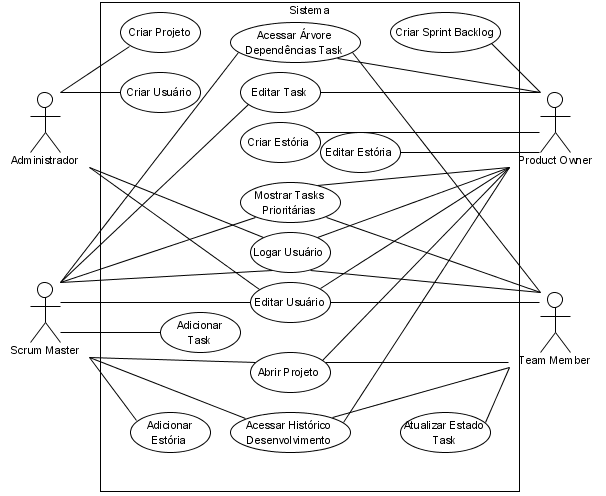
\includegraphics[width=130mm]{diagramas/CasosDeUso.png}
  \caption[casos_de_uso]{Diagrama de Casos de Uso}
  \label{casos_de_uso}
\end{center}
\end{figure}

\subsection{Editar usuário}
\begin{description}
\item[Escopo:] Sistema de Usuários
\item[Nível:] Meta do usuário
\item[Ator Primário:] Usuário

\item[Stakeholders e seus interesses:] \hfill \\ 
Usuário: Deseja editar seu nome ou senha.

\item[Pré-condições:] O usuário está logado com a conta a ser editada.

\item[Pós-condições:] Os dados alterados são armazenados no sistema.

\item[Fluxo Básico ou Cenário Principal:] \hfill
\begin{enumerate}
  \item O usuário informa o campo que deseja alterar
  \item O usuário informa o novo valor do campo a ser alterado
  \item O sistema atualiza as informações do usuário

\end{enumerate}

\item[Extensões:] \hfill
\begin{description}
	\item[2a.] O novo valor fornecido está em branco
		\begin{enumerate}
 			\item O sistema informa o usuário da que o campo não pode ser deixado em
 			branco
  			\item O sitema requisita um novo valor para o campo enquanto esse estiver
  			vazio
		\end{enumerate}
\end{description}
\item[Requisitos especiais:] Nenhum

\item[Tecnologia:] \hfill
\begin{description} 
	\item[2a.] A entrada dos dados é feita pelo teclado.
\end{description}
\item[Freqüência de Ocorrência:] Raramente.

\end{description}


\subsection{Editar Estória}
\begin{description}
\item[Escopo:] Sistema de Edição de Projetos
\item[Nível:] Meta do usuário
\item[Ator Primário:] Product Owner

%TODO: Alterar as tarefas que a estória contém?
\item[Stakeholders e seus interesses:] \hfill \\ 
Product Owner: Deseja poder editar uma estória, alterando seu nome ou descrição.

\item[Pré-condições:] O usuário está logado como Product Owner. O projeto
responsável pela estória está aberto.

\item[Pós-condições:] Os dados alterados são armazenados no sistema.

\item[Fluxo Básico ou Cenário Principal:] \hfill
\begin{enumerate}
  \item O usuário informa o ID da estória a ser alterada
  \item O usuário informa o campo a ser alterado na estória
  \item O usuário informa o novo valor do campo a ser alterado
  \item O sistema atualiza as informações da estória
\end{enumerate}

\item[Extensões:] \hfill
\begin{description}
	\item[1a.] O ID fornecido não existe
		\begin{enumerate}
 			\item O sistema informa o usuário que a estória não existe
 			\item O caso de uso é encerrado.
		\end{enumerate}
\end{description}
\item[Requisitos especiais:] Nenhum

\item[Tecnologia:] \hfill
\begin{description} 
	\item[2-3a.] A entrada dos dados é feita pelo teclado.
\end{description}
\item[Freqüência de Ocorrência:] Raramente.

\end{description}

\subsection{Editar Task}
\begin{description}
\item[Escopo:] Sistema de Edição de Projetos
\item[Nível:] Meta do usuário
\item[Ator Primário:] Product Owner/Scrum Master

%TODO: Alterar os requisitos? Responsável?
\item[Stakeholders e seus interesses:] \hfill \\ 
Product Owner/Scrum Master: Deseja poder editar uma tarefa, alterando seu nome,
descrição, dificuldade ou estimativa.

\item[Pré-condições:] O usuário está logado como Product Owner ou Scrum Master.
O projeto responsável pela task está aberto.

\item[Pós-condições:] Os dados alterados são armazenados no sistema.

\item[Fluxo Básico ou Cenário Principal:] \hfill
\begin{enumerate}
  \item O usuário informa o ID da tarefa a ser alterada
  \item O usuário informa o campo a ser alterado na tarefa
  \item O usuário informa o novo valor do campo a ser alterado
  \item O sistema atualiza as informações da tarefa
\end{enumerate}

\item[Extensões:] \hfill
\begin{description}
	\item[1a.] O ID fornecido não existe
		\begin{enumerate}
 			\item O sistema informa o usuário que a tarefa não existe
 			\item O caso de uso é encerrado.
		\end{enumerate}
\end{description}
\item[Requisitos especiais:] Nenhum

\item[Tecnologia:] \hfill
\begin{description} 
	\item[2-3a.] A entrada dos dados é feita pelo teclado.
\end{description}
\item[Freqüência de Ocorrência:] Raramente.

\end{description}


\subsection{Acessar o histórico do desenvolvimento}
\begin{description}
\item[Escopo:] Sistema de Edição de Projetos
\item[Nível:] Meta do usuário
\item[Ator Primário:] Usuário

%TODO: Isso não faz nada de novo...
\item[Stakeholders e seus interesses:] \hfill \\ 
Usuário: Deseja ter um panorama geral do histórico de desenvolvimento,
apresentando o estado atual das tarefas concluídas e a concluir, e estórias.

\item[Pré-condições:] O projeto cujo histórico deseja ser acessado está aberto.

\item[Pós-condições:] O histórico atual de desenvolvimento do projeto é exibido
ao usuário.

\item[Fluxo Básico ou Cenário Principal:] \hfill
\begin{enumerate}
  \item O usuário requisita a visualização do histórico de desenvolvimento
  \item O sistema apresenta as informações descritas anteriormente.
\end{enumerate}

\item[Extensões:] Nenhuma.
\item[Requisitos especiais:] Nenhum.

\item[Tecnologia:] Nenhuma.
\item[Freqüência de Ocorrência:] Raramente.

\end{description}


\subsection{Acessar árvore de dependências de uma task}
\begin{description}
\item[Escopo:] Sistema de Edição de Projetos
\item[Nível:] Meta do usuário
\item[Ator Primário:] Usuário

\item[Stakeholders e seus interesses:] \hfill \\ 
Usuário: Deseja visualizar a árvore que apresenta todas as dependências de uma
dada tarefa.

\item[Pré-condições:] O usuário está logado e há um projeto aberto.

\item[Pós-condições:] A árvore é apresentada ao usuário.

\item[Fluxo Básico ou Cenário Principal:] \hfill
\begin{enumerate}
  \item O usuário informa o ID da tarefa a ser visualizada
  \item O sistema apresenta a árvore de dependências da tarefa.
\end{enumerate}

\item[Extensões:] \hfill
\begin{description}
	\item[1a.] O ID fornecido não existe
		\begin{enumerate}
 			\item O sistema informa o usuário que a tarefa não existe
 			\item O caso de uso é encerrado.
		\end{enumerate}
\end{description}
\item[Requisitos especiais:] Nenhum

\item[Tecnologia:] \hfill
\begin{description} 
	\item[2a.] A entrada dos dados é feita pelo teclado.
\end{description}
\item[Freqüência de Ocorrência:] Raramente.

\end{description}


\subsection{Mostrar para o usuário quais são tasks prioritárias}
\begin{description}
\item[Escopo:] Sistema de Edição de Projetos
\item[Nível:] Meta do usuário
\item[Ator Primário:] Usuário

%TODO: É esse o critério que vamos adotar?
\item[Stakeholders e seus interesses:] \hfill \\ 
Usuário: Deseja visualizar as tarefas prioritárias (As que são pré-requisito
para a maior quantidade de tarefas).

\item[Pré-condições:] O usuário está logado e há um projeto aberto.

\item[Pós-condições:] A lista de tasks prioritárias é apresentada.

\item[Fluxo Básico ou Cenário Principal:] \hfill
\begin{enumerate}
  \item O usuário requisita a lista de tarefas prioritárias
  \item O sistema apresenta as tarefas em ordem de prioridade.
\end{enumerate}

\item[Extensões:] Nenhuma.
\item[Requisitos especiais:] Nenhum

\item[Tecnologia:] Nenhuma.
\item[Freqüência de Ocorrência:] Raramente.

\end{description}


\chapter{Análise}
\section{Diagrama de Classes Conceituais}


\chapter{Projeto}
\section{Diagrama de Classes}


\section{Diagramas de Interação}
\subsection{Editar usuário}


\subsection{Editar Estória/Task}


\subsection{Acessar o histórico do desenvolvimento}


\subsection{Acessar árvore de dependências de uma task}


\subsection{Mostrar para o usuário quais são tasks prioritárias}


\section{Projeto da Persistência dos Objetos}


\section{Diagrama de Atividades}
\subsection{Diagrama de Atividades 1}


\subsection{Diagrama de Atividades 2}


\section{Statecharts}
\subsection{Statechart 1}


\subsection{Statechart 2}



\end{document}